\documentclass[12pt,a4paper]{article}
\usepackage[utf8]{inputenc}
\usepackage[francais]{babel}
\usepackage[T1]{fontenc}
\usepackage[left=2.5cm,right=2.5cm,top=3cm,bottom=3cm]{geometry}
\usepackage{lipsum}
\usepackage{nccparskip}
\usepackage{setspace}
\usepackage{graphicx}
\usepackage{caption}
\usepackage{fancyhdr}
\usepackage{rotating}
\usepackage{hyperref}

\pagestyle{fancy}
\renewcommand{\headrulewidth}{1pt}
\fancyhead[R]{\textbf{page \thepage}}
\renewcommand{\footrulewidth}{2pt}
\fancyfoot[C]{INSTITUT UNIVERSITAIRE DE TECHNOLOGIE  \\3, rue du Maréchal Joffre 44041 cedex 01 - http://www.iut-nantes.univ-nantes.fr}

\renewcommand{\thesection}{\Roman{section}}
\renewcommand{\thesubsection}{\roman{subsection}}
\renewcommand{\thesubsubsection}{\roman{subsubsection}}

\usepackage{array,multirow,makecell}
\setcellgapes{1pt}
\makegapedcells
\newcolumntype{R}[1]{>{\raggedleft\arraybackslash }b{#1}}
\newcolumntype{L}[1]{>{\raggedright\arraybackslash }b{#1}}
\newcolumntype{C}[1]{>{\centering\arraybackslash }b{#1}}



\begin{document}
\thispagestyle{empty}

\begin{figure}
\begin{minipage}[t]{5cm}
\centering

\includegraphics[scale=0.75]{iutNantes.jpg}
\end{minipage}
\begin{minipage}[t]{15cm}
\centering

\includegraphics[scale=1.3]{logo_UnivNantes.png}
\end{minipage}
\end{figure}

\bigbreak
\bigbreak
\bigbreak
\bigbreak

\begin{center}
\begin{large}
\textbf{INSTITUT UNIVERSITAIRE DE TECHNOLOGIE \bigbreak
Département INFORMATIQUE \bigbreak
(Computer Science Department – Nantes Institute of Technology)
\bigbreak
\bigbreak
\bigbreak
Rapport de Projet Technologique \bigbreak
2015-2016
\bigbreak
\bigbreak
Job Meeting}
\bigbreak
2ème année
\end{large}
\end{center}

\bigbreak
\bigbreak
\bigbreak

\begin{tabular}{C{8cm}L{5cm}}
\textbf{Réalisé par :} & - Nathan MARAVAL \\
 & - Brewal HENAFF\\
 & - Morgane VIAUD\\
 & - Susie ROBIN\\
 & - Lucas CHOQUET\\
\textbf{Client(s) :} & Tifenn CORBEL\\
\textbf{Encadré par :} & Abdelghani HADJ-RABIA
\end{tabular}

\bigbreak
\bigbreak
\bigbreak

\begin{center}\begin{large}
\textbf{du 28/09/15 au 31/03/2016}

\newpage

\textbf{Agenda des phases du travail}
\end{large}\end{center}

\bigbreak
\bigbreak
\bigbreak

\begin{tabular}{|L{5cm}|C{3cm}|L{5cm}|}
\hline \textbf{Phases} & \textbf{Dates} & \textbf{Commentaires} \\
\hline Réunion de démarrage (avec encadrant) & 01/10/2015 & Mise en place du projet avec A. Hadj-Rabia et T. Corbel \\
\hline Réunion sur cahier des charges & 04/11/2015 &  \\
\hline Réunion sur l’avancement du projet & 03/12/2015 & Finir les bases de données \\
\hline Réunion sur l’avancement du projet & 17/12/2015 & Faire des tests pour l’algorithme  avec des données \\
\hline Réunion sur l’avancement du projet & 14/01/2015 & Mise en place du lien entre l’algorithme et la base de donnée \\
\hline Récupération du rapport par l'encadrant & 18/01/2016 & \\
\hline Soutenance orale pour présenter le projet & 21/01/2016 & \\
\hline
\end{tabular}

\newpage
\vspace*{\stretch{1}}
\begin{large}
\begin{onehalfspace}
Résumé (en français) : Dans le cadre de l’événement Job Meeting organisé par l’IUT de Nantes pour permettre à des étudiants de rencontrer des entreprises dans l’éventualité d’obtenir un contrat d’alternance, il nous a été demandé de réaliser une application web permettant de générer les emplois du temps relatifs aux rencontres de l’événement avec efficience. L’objectif est de passer de la génération “à la main” à une génération automatisée, bien moins laborieuse.

\bigbreak
\bigbreak
\bigbreak
\bigbreak
\bigbreak
\bigbreak
\bigbreak

\textit{Abstract (résumé en Anglais): With the approach of the Job Meeting event organized by Nantes’ University, we have been asked to set up a web application that would generate easily the schedules linked with the meetings of this event. The Job Dating event consists into helping students to meet companies so they can try to discuss about a study contract. The objective of this project is to let aside the hand-made schedule creation in order to use an automatic generation of these schedules.}\end{onehalfspace}
\end{large}
\vspace*{\stretch{1}}
\newpage
\renewcommand{\contentsname}{Sommaire}
\tableofcontents
\newpage
\section{Présentation du sujet}

\begin{large}
\begin{onehalfspace}Le 1 Avril 2015 se déroulera un évènement, à Carquefou. Nommé Job Meeting, il permettra aux étudiants en recherche de contrats d’alternance de rencontrer des recruteurs d’entreprises correspondant à leurs attentes et à leur formation originelle.

	Tifenn CORBEL, Responsable des Relations Entreprises, nous propose de réaliser tout le site lié au Job Meeting dans le but de l’utiliser pour gérer les inscriptions des entreprises et des étudiants à l’évènement et leur afficher leur emploi de temps des rencontres de la journée.

	L’un des buts principaux de ce projet, en plus de la création du site, est de pouvoir proposer des emplois du temps générés grâce à un algorithme aux participants du Job Meeting. Avant de faire appel à nous, les années précédentes, il fallait faire les emplois du temps à la main ; ce qui demandait beaucoup de temps d’arrachage de cheveux pour trouver un moyen de faire concorder les voeux de chaque étudiants avec les entreprises disponibles. De ce fait, grâce à cet algorithme, il serait possible de réaliser des modifications de dernières minutes en quelques instants, ce qui était impensable à cause des nombreuses heures passées pour établir les emplois du temps avant la date prévue du Job Meeting.
\end{onehalfspace}
\end{large}


\newpage
\section{Analyse du sujet}

\begin{large}
\begin{onehalfspace}Avant de nous lancer dans la programmation, nous avons analysé attentivement notre sujet de projet pour établir ce qui nous était nécessaire de réaliser pour arriver à un site web complet et opérationnel. Nous avons réalisé un diagramme de cas d’utilisation (voir figure 1 page 17), qui a dû légèrement être modifié depuis le début du projet, pour nous aider dans la conception de notre site.

	Pour cela, nous avons réfléchi sur deux points très importants ; il s’agit de l’inscription des entreprises et celle des étudiants ainsi que la manière de générer des emplois du temps.

	L’organisation de la journée du Job Meeting se faisait suivant la figure 2 (page 18), en plusieurs étapes qu’il était essentiel de séparer ; pour notamment ne pas mélanger les inscriptions des entreprises et des étudiants. Pour notre projet, nous avons repris ces étapes en les automatisant ; c’est-à-dire en rendant la réalisation des emplois du temps plus rapide à l’aide d’un algorithme et en rendant l’inscription à l’évènement plus simple grâce à un formulaire d’inscription.
\end{onehalfspace}
\end{large}


\subsection{Les inscriptions}

\begin{large}
\begin{onehalfspace}Concernant les inscriptions sur notre site, il nous a été indiqué qu’elles s’effectueraient grâce à un formulaire spécifique pour les étudiants et les entreprises.

    Pour les entreprises, leur formulaire contiendrait des indications sur le nombres de personnes qui viendront pour recruter  pendant le Job Meeting. Des questions par rapport aux repas sont également posées pour pouvoir organiser au mieux la journée. Les entreprises devront indiquer les formations dans lesquelles elles souhaitent recruter ainsi que le nombre d’étudiants qu’elles souhaitent recruter. Concernant les étudiants, leur formulaire contiendrait des indications concernant leur formation et leurs coordonnées.
\end{onehalfspace}
\end{large}

\subsection{La génération de emplois du temps}

\begin{large}
\begin{onehalfspace}    Les emplois du temps étaient fait à la main et prenaient beaucoup de temps à être fait. On appliquait une version manuelle de l’algorithme des huit reines qui consistaient à placer un élément dans l’emploi du temps et de placer les autres en fonction de celui-ci en veillant à ce qu’une ligne, colonne et diagonale ne soit occupée que par un seul élément. Cependant, cet algorithme prenait beaucoup de temps car lorsqu’un élément ne concordait pas, il fallait retourner en arrière pour déplacer des éléments et trouver une solution.

    De ce fait, notre principal objectif est de retranscrire l’algorithme des huit reines en programme informatique qui sera capable de générer un emploi du temps avec des données passées en paramètre de façon automatique. L’algorithme prendra en compte les voeux des étudiants, le nombre de créneaux disponibles et les disponibilités de l’entreprise. Le but est d’obtenir un rendu plus ou moins similaire à la figure 3 (page 19).

\end{onehalfspace}
\end{large}

\subsection{Les différents types de comptes du site}

\begin{large}
\begin{onehalfspace}    Pour réaliser ce type de site, il nous est nécessaire d’avoir différentes vues en fonction de qui se connecte. En effet, lors de son inscription, une entreprise ne va pas avoir à remplir le même formulaire qu’un étudiant. De ce fait, si une entreprise souhaite modifier des données de son formulaire, elle devra pouvoir y accéder sur sa page après s’être connectée.

    Ainsi nous avons créé trois types de comptes différents qui vont chacun avoir une vue du site adaptée à son statut. Les étudiants et les entreprises ne pourront voir que les éléments qui leur seront spécifiques ; en revanche, l’administrateur aura une vue bien plus large.

    L’administrateur devra être capable de voir tous les utilisateurs. Lorsqu’une entreprise ou un étudiant s’inscrira, il devra attendre que l’administrateur valide son compte. Le compte peut également être gelé ou encore supprimé par l’administrateur.

    L’administrateur devant effectuer les mêmes actions pour les entreprises et les étudiants, nous avons choisi de le représenter sur les diagrammes de cas d’utilisation d’un étudiant et d’une entreprise. Les figures 4 et 5(page 20) représentent les actions que peuvent faire respectivement un étudiant et une entreprise sur le site.
\end{onehalfspace}
\end{large}
\newpage
\section{Réalisation du projet}

\begin{large}
\begin{onehalfspace}    La réalisation de projet s’effectue en trois temps. Tout d’abord, nous avons réfléchi au visuel du site et à son développement; ensuite il a fallu coder les différents scripts nécessaires pour pouvoir naviguer sur notre site ; et enfin, nous avons fait la base de données qui sera indispensable pour les inscriptions
\end{onehalfspace}
\end{large}

\subsection{Le site Web}

\begin{large}
\begin{onehalfspace}Le site est la partie visuelle de notre projet. Elle a été pensée et réfléchie pour être la plus simple d’utilisation possible.
\end{onehalfspace}
\end{large}

\subsubsection*{Le Modèle MVC}

\begin{large}
\begin{onehalfspace}Le modèle MVC (Modèle Vue Contrôleur) est un modèle permettant une forte adaptabilité à de nombreuses situations. Il permet aussi d’éviter une hiérarchie sous la forme d’un arbre très imposant et de contrôler plus aisément les interactions entre les différents éléments du site, y compris l’utilisateur.

    Le Modèle MVC peut se schématiser comme cela :

      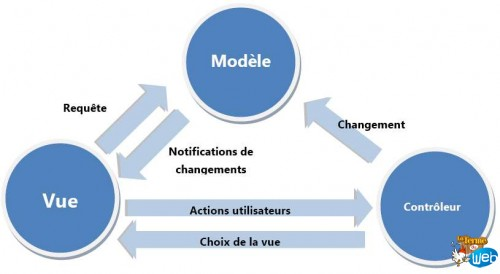
\includegraphics[scale=0.5]{figure6(3_1).png}


    L’utilisateur a devant lui uniquement la vue. La vue acquiert les actions de l’utilisateur et a accès à des contrôleurs qui déterminent l’action à réaliser. Si la vue a besoin d’afficher des données provenant d’une source externe, celle-ci demande au modèle de données de les lui envoyer. De cette manière, le modèle indique à la vue les données à afficher.

    Les contrôleurs vont déterminer quelle vue afficher selon les choix de l’utilisateur, les données, etc, et va interagir avec le modèle de données pour le modifier.
\end{onehalfspace}
\end{large}

\subsubsection*{Les formulaires}

\begin{large}
\begin{onehalfspace}Les formulaires d’inscription sont codés en HTML, CSS et JQuery pour l’affichage et en javascript pour la gestion des champs d’input. Le javascript est utilisé pour déterminer si les valeurs entrées dans les champs par l’utilisateur sont celles attendues par le système. De plus nous avons mis une double sécurité à ce niveau là : une couche dynamique et une en dur dans le code. La couche dynamique en javascript va amener un confort d’utilisation : en cas de valeur erronée, il est demandé à l’utilisateur d’entrer une nouvelle valeur et on vérifiera si celle-ci est correcte ou toujours incorrecte. Cependant le javascript peut être désactivé par l’utilisateur, ce n’est donc pas une sécurité fiable pour notre site.

	On va alors vérifier encore une fois toutes les données au moment de l’envoie avec du formulaire. Un script PHP qui va alors les traiter, ce qui nous permet d’avoir forcément nos tests. On va notamment regarder si l’entreprise ou l’étudiant existe déjà ou si son compte est validé ou en attente de validation. Ayant un accès direct à la base de données, une inscription validée sera ajoutée dans l’état d’attente de validation.
\end{onehalfspace}
\end{large}

\subsubsection*{Le design général}

\begin{large}
\begin{onehalfspace}Le site internet sera la plate-forme entre les participants à l’événement Job Meeting et l’application web qui stockera les données et générera les emplois du temps. La page d’index propose à l’utilisateur de se connecter, de s’inscrire selon son statut (étudiant ou entreprise) et éventuellement de demander à ce que son mot de passe soit réinitialisé. Une fois connecté, un utilisateur régulier pourra accéder au planning (si celui-ci est généré), modifier les paramètres de son compte, demander à ce que celui-ci soit gelé, se déconnecter. Un étudiant pourra choisir jusqu’à quatre entreprises à rencontrer, et une entreprise pourra gérer ses stands. Le site internet utilise le modèle MVC car celui-ci permet de générer un site web avec une hiérarchie concrète et organisée.

    Les figures 7 à 11 (page 21 à 23) sont des captures d’écran de différentes pages du site déployé.
\end{onehalfspace}
\end{large}

\subsection{La base de données}

\begin{large}
\begin{onehalfspace}    La base de données du site est indispensable pour pouvoir enregistrer les inscriptions des utilisateurs. De ce fait, nous avons créé plusieurs tables avec 2 idées en tête : conserver les informations sur les comptes des entreprises et des étudiants et avoir toutes les données nécessaires à la génération des emplois du temps. (Figure 6 page 21)

    Pour les comptes entreprises et étudiants on a mis 2 type de tables en places. Les tables “entreprise” et “etudiant” vont contenir toutes les informations sur les comptes enregistrés. On a aussi les tables “temp\_etudiant” et “temp\_entreprise” qui vont regrouper les comptes qui n’ont pas encore été validés. Ils vont dans un second temps être transférés dans les tables principales, on évite absolument les doublons. La table “identificationadmin” va servir à stocké les informations de connexion des administrateurs.

    A partir de la table entreprise on va générer les différents créneaux d'entretiens dans la table formation. Chaque formation va représenté un recruteur de l’entreprise sur une formation et une tranche horaire. Ainsi la table formation est lié à pour clé secondaire la table entreprise. Enfin la table creneau va contenir tous les entretiens de la journée, avec l’horaire associé. Pour cela, un créneau va être lié avec un étudiant et une formation.

	Ces tables sont stockées sur une base de données MySQL, de ce fait, elles sont facilement accessibles à travers le code PHP et par l’outil PHPMyAdmin.
\end{onehalfspace}
\end{large}

\subsection{Les scripts}

\begin{large}
\begin{onehalfspace}Présents sur le routeur, sur les contrôleurs et sur le fichier de connexion à la base de données, les scripts, codés en PHP, permettent de réaliser les tâches que l’application web doit réaliser pour pouvoir stocker et utiliser les données relatives à la génération des emplois du temps. Les données sont stockées à travers les formulaires d’inscriptions et utilisées dès qu’une action requiert des données stockées dans la base de donnée. Un peu de javascript est aussi utilisé sur certaines pages contenant des formulaires en HTML.
\end{onehalfspace}
\end{large}

\subsubsection*{Les formations}

\begin{large}
\begin{onehalfspace}L’algorithme de génération de formation, permet de faire l’association entre les formations d’une entreprises et les créneaux disponibles. Ce script répartit les formations recherchées par l’entreprise sur ses créneaux de présence en prenant également en compte le nombre de personne disponible, avec une répartition la plus équitable possible. Il faut ensuite l’ajout dans la base de donnée et nous permet ainsi de faire un affichage comme dans la figure suivante :

  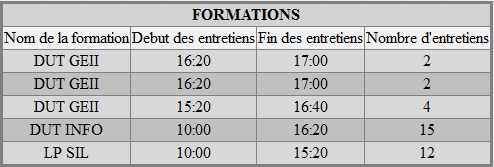
\includegraphics[scale=0.68]{figure9(3_5).jpg}

	Ici chaque ligne correspond à un ensemble d’entretien (nombre indiqué à la fin), pour une formation donnée, qui seront mené par une personne. Les horaires indiques le début et la fin des entretiens cumulé.
\end{onehalfspace}
\end{large}

\subsubsection*{Les emplois du temps}

\begin{large}
\begin{onehalfspace}La génération de l’emploi du temps ce base sur l’algorithme des 8 reines. Le problème des 8 reines est simple, il faut placer 8 reines sur un échiquier de façon à ce qu’elles ne soient pas sur la même ligne horizontale, verticale et diagonales. La figure suivante est un exemple de deux solutions possibles :

  
\includegraphics[scale=0.5]{figure10(3_6).png}

	Ce problème est très simple en apparence, seulement il y a 648 possibilités, soit 281 474 976 710 656 cas. Ainsi il est impensable de toutes les parcourir pour tomber sur une des 92 solutions. Pour y remédier on peux déjà mettre en place les contraintes pour éviter de tester les cas inutiles. Dans le cas suivant, les contraintes sont plus simples :

    
\includegraphics[scale=0.5]{figure11(3_7).jpg}

    Donc dans un premier temps on place les 8 reines en respectant ces contraintes, puis quand on se retrouve dans une impasse on met en place un système de backtracking. C’est à dire on revient en arrière jusqu’au déblocage en se souvenant des précédentes tentatives. Cette méthode est adapté à notre demande qui a moins de contraintes et ce n’est pas gênant d’avoir un programme qui prends du temps.

Dans notre cas on a 3 contraintes :
Un étudiant ne peut avoir qu’un entretient à la fois.
Un étudiant doit avoir un créneau de pause entre chaque entretient
Un étudiant ne peut voir qu’une fois une entreprise

    Avec ce principe on va donc pouvoir placer tous les étudiants. Il s’agit aussi d’équilibrer les entretiens des étudiants. Pour cela on met en place un système de priorité : si un étudiant n’a pas pu avoir son choix n, alors il est prioritaire sur le choix n+1. Ainsi il s’agit simplement de placer les étudiants dans l’ordre de priorité, ce qui ne change rien à notre algorithme.
\end{onehalfspace}
\end{large}

\subsection{La sécurité du site internet}

\begin{large}
\begin{onehalfspace}Le site web va être mis en ligne sur les serveurs de l’université de Nantes. Nous avons déjà parlé de la sécurité de nos formulaires, mais ils existent de nombreuses attaques subtiles et connues. Dans ces conditions il va falloir mettre en place des sécurités pour prévenir les dangers suivants :
un abus de confection
attaque sur les serveurs et base de données
manipulation et récupération des données…

    Pour vacciner notre site, il va falloir s’occuper de chaque attaque possible. Tout d’abords on s’est occupé des injections SQL, qui est une attaque simple sur les bases de données. Il s’agit d’injecter une requête SQL non prévu par le système pour le manipuler. Le plus classique serait de taper (‘ OR 1 = 1) à la place de son login pour passer les conditions de vérifications. Pour y parer nous avons mis en place un échappement des caractères spéciaux. C’est à dire on a géré tous les caractères spéciaux liées au SQL, en les transformant. Cette méthode est à appliqué sur tous les zones de saisie de texte (notamment nos formulaire).

	Le Cross Site Scripting, abrégé XSS (Cross voulant dire “croix” en anglais, le symbole X a été choisi pour le représenter), est un type de faille de sécurité que l'on trouve typiquement dans les applications web. Le principe consiste à injecter du code (html, javascript ...) directement dans les pages web. Cela se fait généralement via un formulaire à remplir, en déposant un message dans un forum, dans un moteur de recherche ou directement dans l'URL d'un site, en y ajoutant quelques paramètres.

	Une première solution pour contrer ces attaques, est tout simplement d'interdire l'utilisation de la balise html <script>. Mais cela n'est pas suffisant, car on peut contourner facilement la protection en utilisant d'autres balises html, comme la balise iframe :

    <iframe src=“http://site-du-hacker.com”></iframe>

	Il est donc plus prudent d'interdire toute utilisation de balises html.

	Pour toutes les attaques n’utilisant pas de balises html ou utilisant une image, avec un “onerror”, nous n’avons pas mis en place de protection, celle-ci étant assez compliquer à mettre en place.
\end{onehalfspace}
\end{large}

\section{Conclusion}

\begin{large}
\begin{onehalfspace}    Le projet était très complet en matière de développement. En effet, nous devions concevoir le site web de A à Z en utilisant nos connaissances acquises en cours pour réussir. Ainsi, nous avons pu savoir plus précisément comment allier le code html du site avec le PHP et le SQL des scripts et bases de données pour créer un site fonctionnel.

    De plus, nous avons travaillé dans de véritables conditions de projet car nous avons une deadline réelle. De ce fait, notre site était fonctionnel pour la date d’ouverture des inscriptions aux entreprises et la génération des emplois du temps est opérationnelle pour le jour du Job Meeting.

    Il était intéressant de travailler avec un client non initié à l’informatique qui nous demandait ce qu’il souhaitait pour le site et nous posait des conditions et contraintes précises ce qu’il voulait. Nous devions faire notre possible pour adapter le langage parlé en langage informatique pour obtenir ce que le client avait en tête.
\end{onehalfspace}
\end{large}

\section{Perspectives d'évolution}

\begin{large}
\begin{onehalfspace}Pour permettre à notre projet d’évoluer davantage, il est envisageable de  créer une application mobile qui permettrait aux étudiants et aux entreprises d’avoir leur planning en temps réel et d’être informés en cas de changement de dernière minute. Cela pourrait être un sujet pur un futur projet.

	De plus, il est tout à fait envisageable d’améliorer l’aspect visuel du site pour le rendre plus attrayant, et plus intuitif. Ainsi que rajouter la possibilité pour l’utilisateur de pouvoir télécharger son planning au format CSV, ICS ou encore PDF.
\end{onehalfspace}
\end{large}

\appendix
\vfill
\section{Annexes}

% diagamme CU
\begin{sidewaysfigure}
  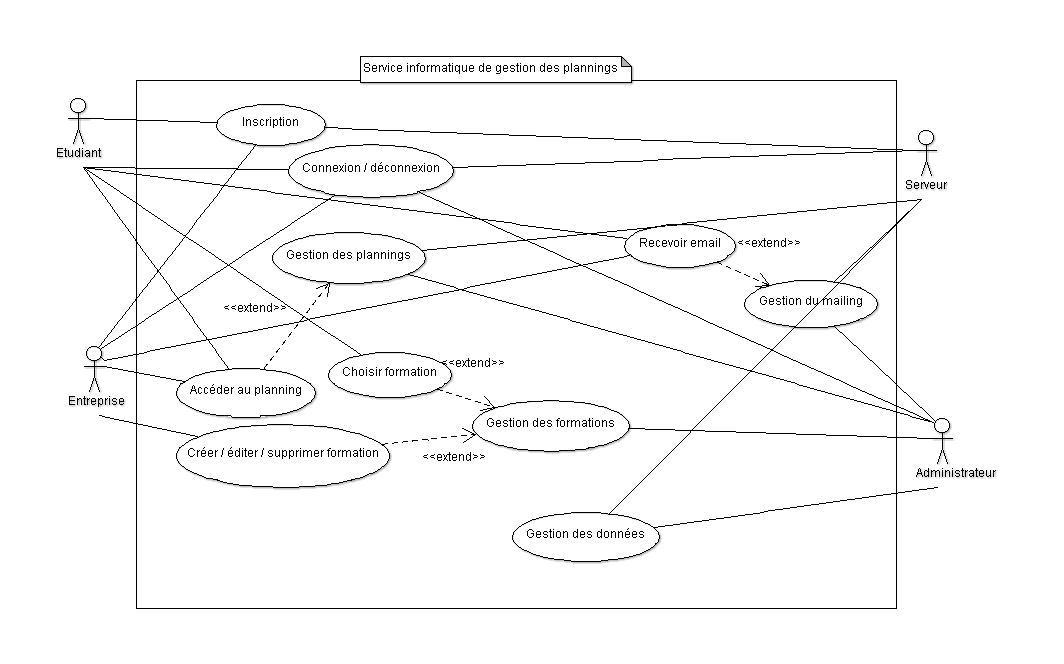
\includegraphics[scale=0.68]{CasUtilisation.png}
  \captionof{figure}{2\_1 Diagramme de Cas d'Utilisations}
\end{sidewaysfigure}

% joli dessin
\begin{sidewaysfigure}
  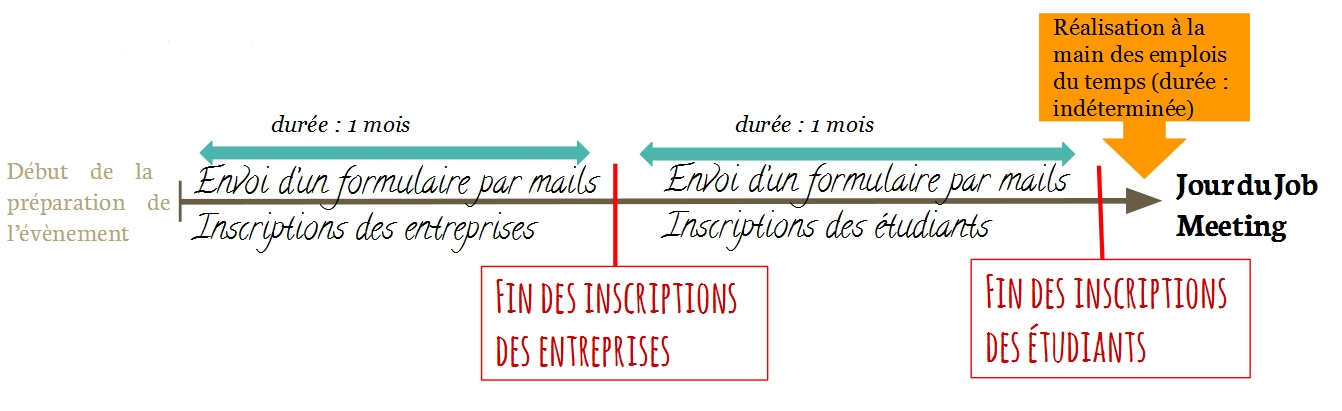
\includegraphics[scale=0.68]{figure2(2_2).jpg}
  \captionof{figure}{2\_2 Schéma des différents états de l'inscription}
\end{sidewaysfigure}

% planning fais a la main
\begin{sidewaysfigure}
  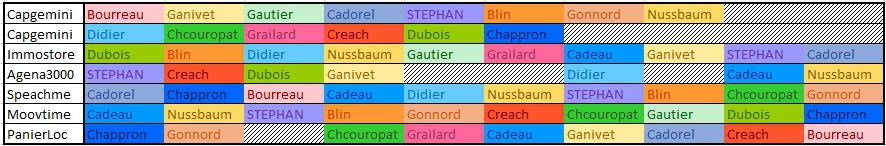
\includegraphics[scale=0.68]{figure3(2_3).jpg}
  \captionof{figure}{2\_3 Planning dais à la main}
\end{sidewaysfigure}

% cas d'utilisation + modèle mvc
\begin{figure}
  \centering
  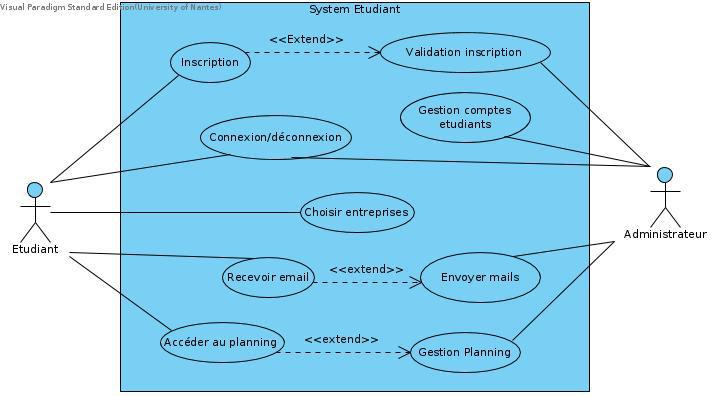
\includegraphics[scale=0.5]{figure4(2_3).jpg}
  \captionof{figure}{2\_3 Diagramme de cas d'utilisation étudiant}
  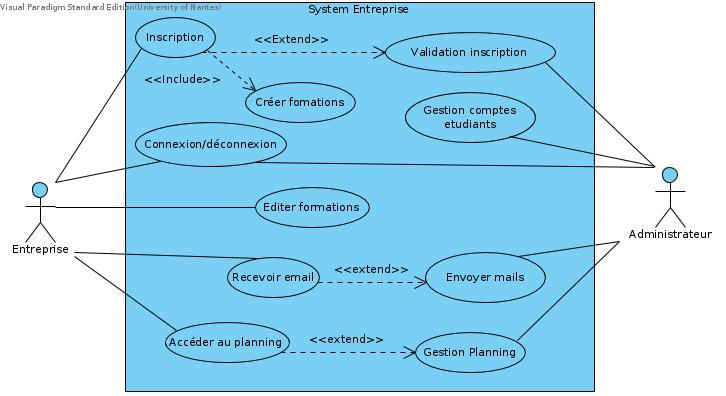
\includegraphics[scale=0.5]{figure5(2_4).jpg}
  \captionof{figure}{2\_4 Diagramme de cas d'utilisation entreprise}
\end{figure}

\begin{figure}
  \centering
  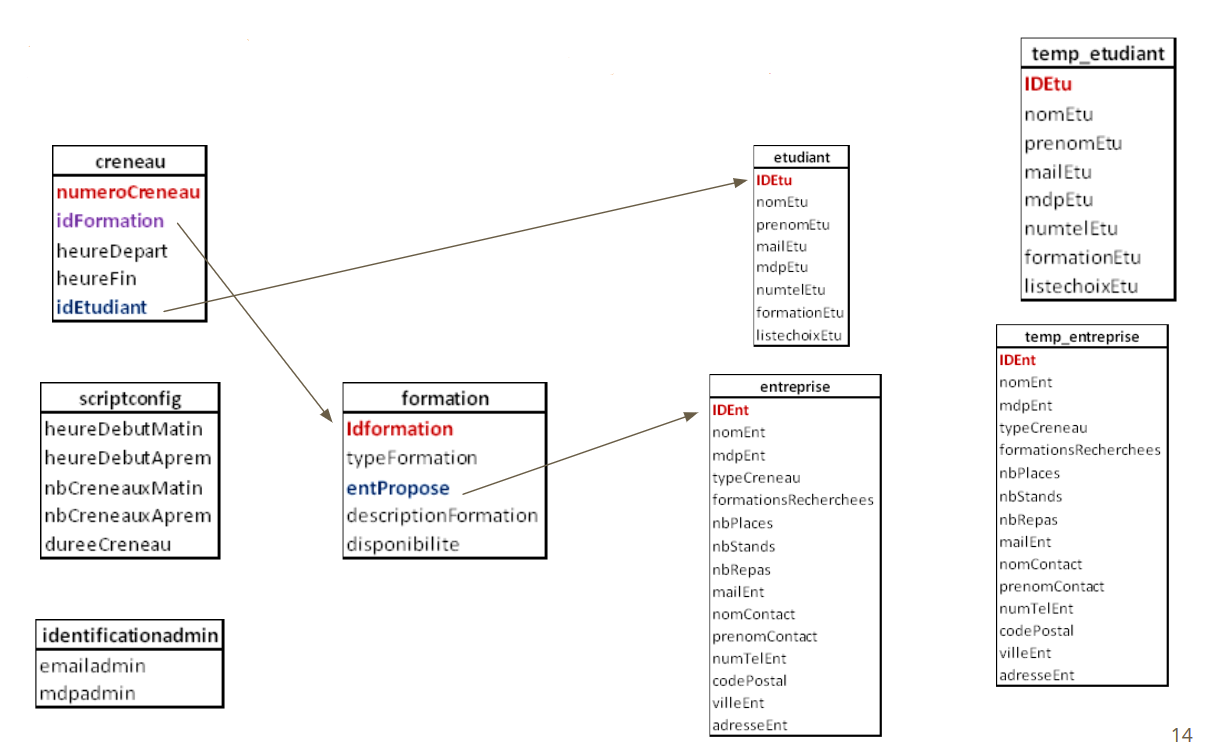
\includegraphics[scale=0.38]{figure12(3_4).png}
  \captionof{figure}{3\_4 Diagramme de classe base de données}
  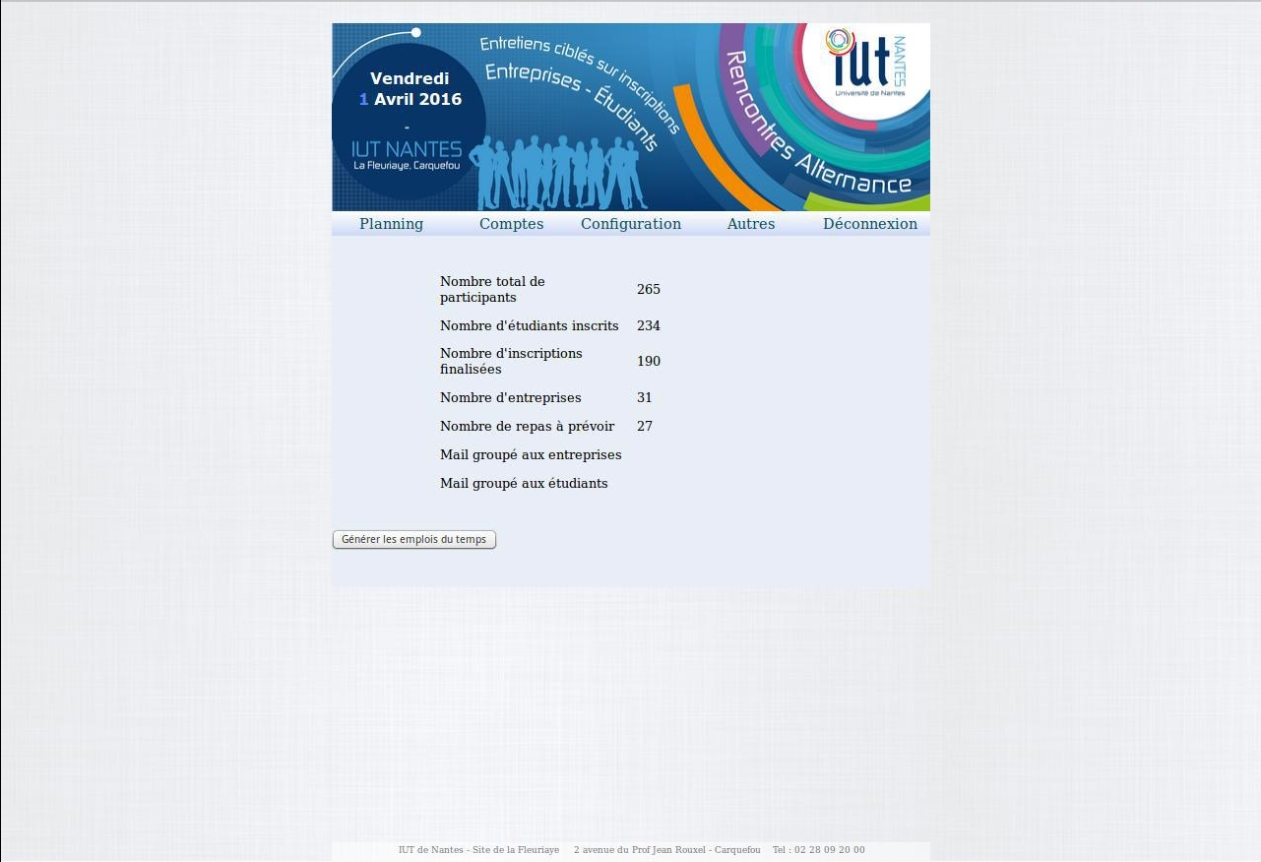
\includegraphics[scale=0.4]{figure7(3_2).jpg}
  \captionof{figure}{3\_2 Page Autre}
\end{figure}

\begin{figure}
  \centering
  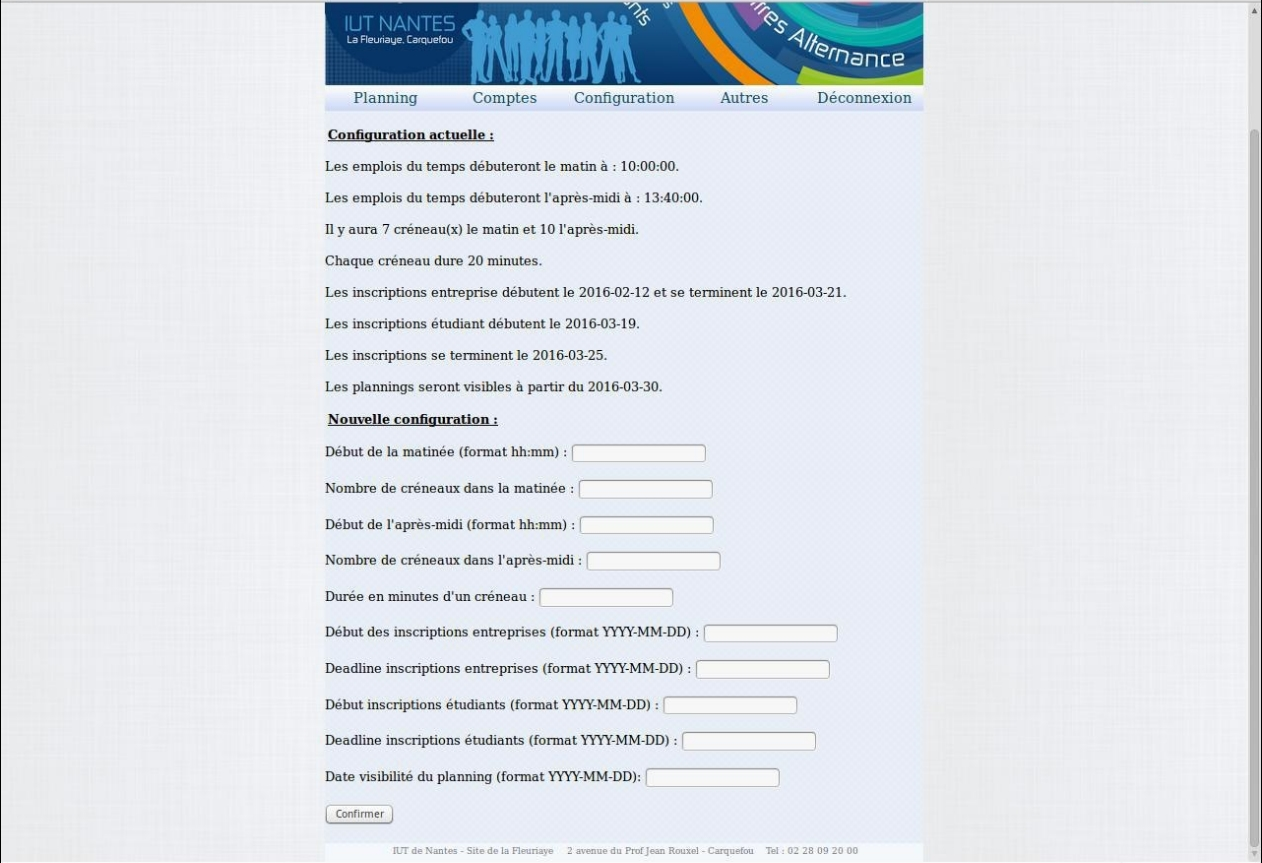
\includegraphics[scale=0.4]{figure8(3_3).jpg}
  \captionof{figure}{3\_3 Page Configuration}
  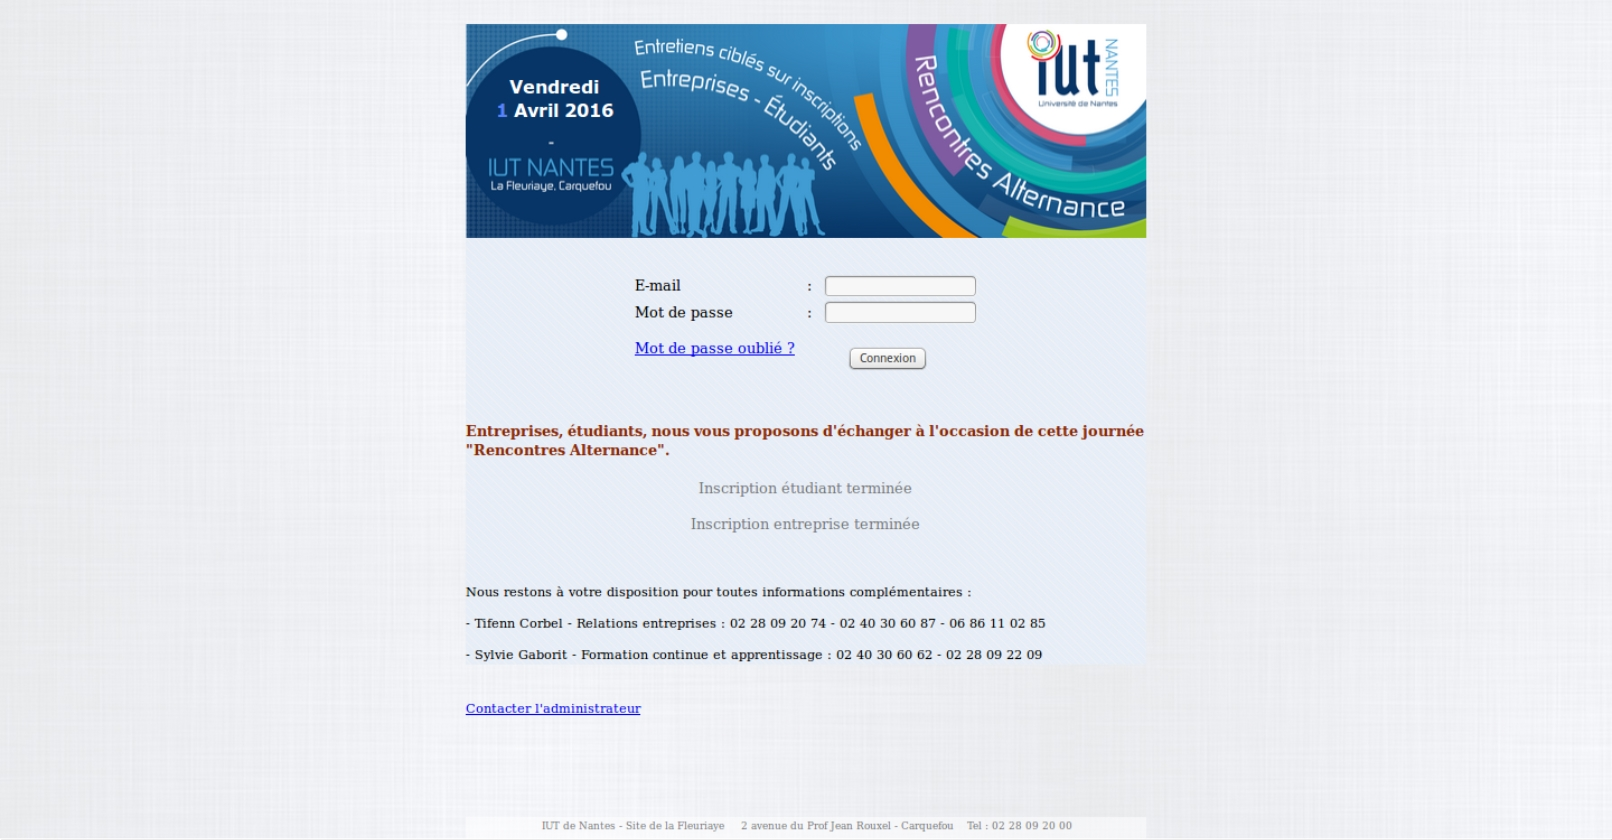
\includegraphics[scale=0.4]{figure13(3_2).jpg}
  \captionof{figure}{3\_3 Page Connexion}
\end{figure}
\begin{figure}
  \centering
  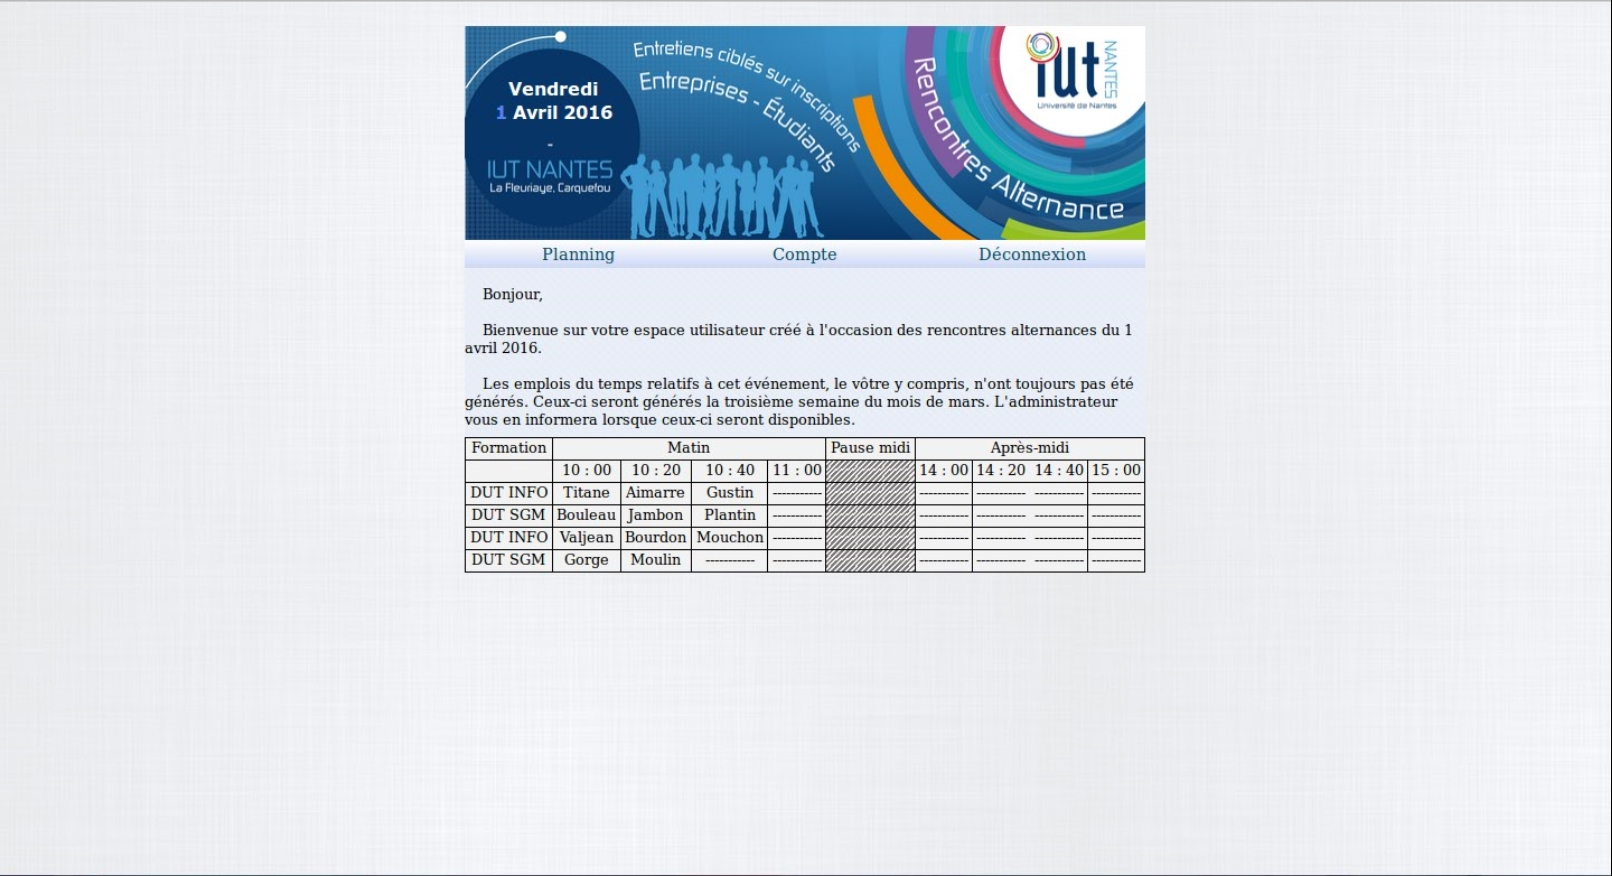
\includegraphics[scale=0.4]{figure14(3_2).jpg}
  \captionof{figure}{3\_3 Page Planning Etudiant}
  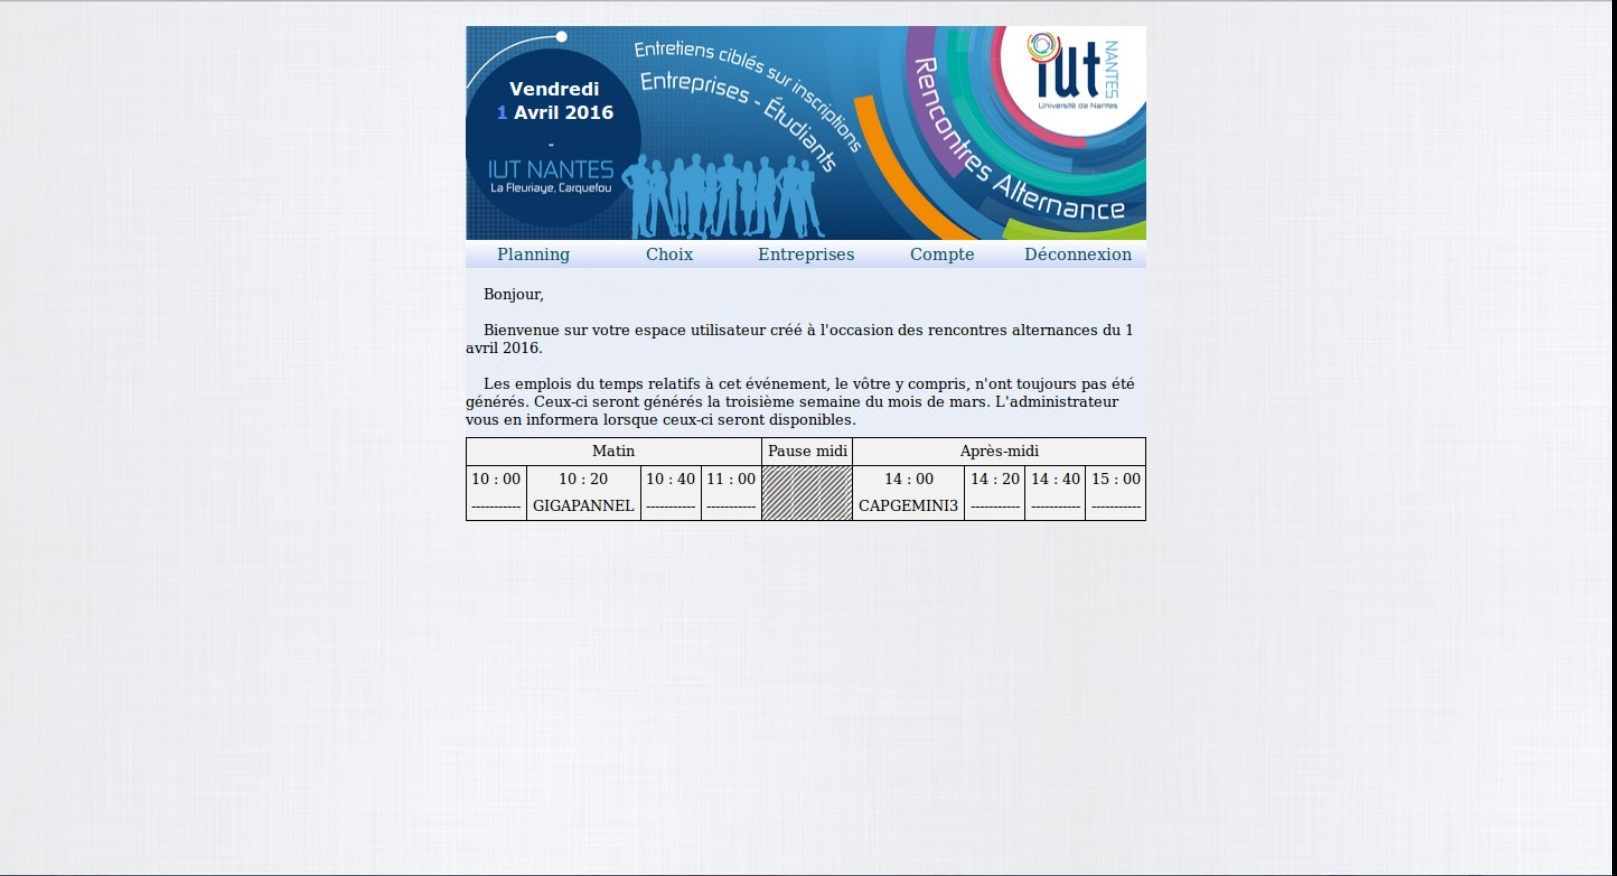
\includegraphics[scale=0.4]{figure15(3_2).jpg}
  \captionof{figure}{3\_3 Page Planning Entreprise}
\end{figure}

\newpage
\begin{center}\begin{huge}\textbf{Rapport de Projet Technologique}\end{huge}


\vfill

\begin{LARGE}\textbf{Université de Nantes}\end{LARGE}
\bigbreak
\begin{LARGE}\textbf{Institut Universitaire de Technologie}\end{LARGE}
\bigbreak
\begin{LARGE}\textbf{Département Informatique}\end{LARGE}


\vfill

\begin{LARGE}\textbf{Nantes, le 18/01/2016}\end{LARGE}
\end{center}
\end{document}
